\documentclass[12pt,a4paper]{article}
%\usepackage[utf8]{inputenc}
%\usepackage[vietnamese]{babel}
\usepackage{amsmath, amsfonts, amssymb}
\usepackage{graphicx}
\usepackage{hyperref}
\usepackage{booktabs}
\usepackage{geometry}
\usepackage{tikz}
\usetikzlibrary{arrows.meta,calc,decorations.pathmorphing,patterns,positioning}
\geometry{left=3cm, right=2cm, top=2.5cm, bottom=2.5cm}

\title{\textbf{TIỂU LUẬN: TÍCH PHÂN VÀ ỨNG DỤNG TRONG THỰC TIỄN}}
\author{\textbf{Sinh viên thực hiện:} [Họ và tên Sinh viên] \\ \textbf{Mã số sinh viên:} [MSSV] \\ \textbf{Lớp:} [Tên Lớp]}
\date{\today}

\begin{document}

\maketitle
\newpage

\tableofcontents
\newpage

\section*{Lời mở đầu}
\addcontentsline{toc}{section}{Lời mở đầu}
Tích phân là một trong những khái niệm nền tảng và quan trọng nhất của Giải tích toán học. Không chỉ dừng lại ở những công thức lý thuyết trừu tượng, tích phân đóng vai trò là một công cụ mạnh mẽ được ứng dụng rộng rãi trong nhiều lĩnh vực của đời sống thực tiễn từ hình học, vật lý, cơ học cho đến kinh tế học và kỹ thuật. Tiểu luận này được thực hiện nhằm hệ thống hóa lại các cơ sở lý thuyết toán học của tích phân, đồng thời đi sâu vào phân tích các ứng dụng thực tế sinh động, giúp người đọc có cái nhìn toàn diện và trực quan hơn về bộ môn khoa học này.

\newpage

\section{Chương 1: Cơ sở lý thuyết của Tích phân}

\subsection{1.1 Định nghĩa Tích phân bất định}
Cho hàm số $f(x)$ xác định trên một khoảng $K$. Hàm số $F(x)$ được gọi là một nguyên hàm của $f(x)$ trên $K$ nếu $F'(x) = f(x)$ với mọi $x \in K$.
Tập hợp tất cả các nguyên hàm của $f(x)$ được gọi là tích phân bất định của $f(x)$, ký hiệu là:
\begin{equation}
\int f(x) \, dx = F(x) + C
\end{equation}
Trong đó $C$ là hằng số tùy ý.

\subsection{1.2 Định nghĩa Tích phân xác định (Tích phân Riemann)}
Cho hàm số $f(x)$ liên tục trên đoạn $[a, b]$. Chia đoạn $[a, b]$ thành $n$ đoạn nhỏ bởi các điểm chia: $a = x_0 < x_1 < \dots < x_n = b$. Trên mỗi đoạn $[x_{i-1}, x_i]$, lấy một điểm $\xi_i$ bất kỳ. Ký hiệu $\Delta x_i = x_i - x_{i-1}$. 
Nếu giới hạn của tổng Riemann:
\begin{equation}
I = \lim_{\max \Delta x_i \to 0} \sum_{i=1}^{n} f(\xi_i) \Delta x_i
\end{equation}
tồn tại và không phụ thuộc vào cách chia đoạn cũng như cách chọn điểm $\xi_i$, thì giới hạn đó được gọi là tích phân xác định của hàm số $f(x)$ trên đoạn $[a, b]$, ký hiệu là:
\begin{equation}
\int_{a}^{b} f(x) \, dx
\end{equation}

\subsection{1.3 Định lý Newton-Leibniz}
\begin{center}
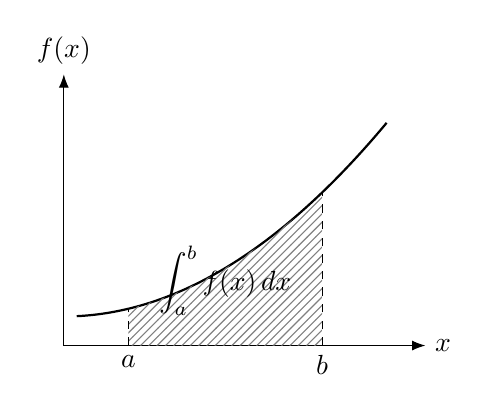
\begin{tikzpicture}[scale=0.82]
    \draw[-{Latex}] (0,0) -- (5.6,0) node[right] {$x$};
    \draw[-{Latex}] (0,0) -- (0,4.2) node[above] {$f(x)$};
    \draw[thick,domain=0.2:5.0,samples=100] plot (\x,{0.45+0.12*\x*\x});
    \path[pattern=north east lines,pattern color=gray]
        (1,0) -- (1,0.57)
        -- plot[domain=1:4,samples=80] (\x,{0.45+0.12*\x*\x})
        -- (4,0) -- cycle;
    \draw[dashed] (1,0) -- (1,0.57);
    \draw[dashed] (4,0) -- (4,2.37);
    \node[below] at (1,0) {$a$};
    \node[below] at (4,0) {$b$};
    \node at (2.5,1.0) {$\displaystyle\int_a^b f(x)\,dx$};
\end{tikzpicture}
\end{center}
Nếu hàm số $f(x)$ liên tục trên đoạn $[a, b]$ và $F(x)$ là một nguyên hàm của $f(x)$ trên $[a, b]$ thì:
\begin{equation}
\int_{a}^{b} f(x) \, dx = F(b) - F(a) = F(x) \Big|_{a}^{b}
\end{equation}

\subsection{1.4 Các phương pháp tính tích phân cơ bản}
\begin{itemize}
    \item \textbf{Phương pháp đổi biến số:} Đặt $x = \varphi(t)$ hoặc $t = \psi(x)$ để đưa tích phân phức tạp về dạng cơ bản hơn.
    \item \textbf{Phương pháp tích phân từng phần:} Dựa trên công thức đạo hàm của một tích:
    \begin{equation}
    \int u \, dv = uv - \int v \, du
    \end{equation}
\end{itemize}

\subsubsection*{Ví dụ 1: Đổi biến số}
Tính tích phân
\[
I=\int 2x\sqrt{x^2+1}\,dx.
\]
Đặt $u=x^2+1$ thì $du=2x\,dx$. Do đó:
\[
I=\int \sqrt{u}\,du
=\frac{2}{3}u^{3/2}+C
=\frac{2}{3}(x^2+1)^{3/2}+C.
\]

\subsubsection*{Ví dụ 2: Tích phân từng phần}
Tính tích phân
\[
I=\int x e^x\,dx.
\]
Chọn $u=x$, $dv=e^x\,dx$, suy ra $du=dx$ và $v=e^x$. Áp dụng công thức tích phân từng phần:
\[
I=xe^x-\int e^x\,dx
=e^x(x-1)+C.
\]

\subsubsection*{Ví dụ 3: Tích phân xác định bằng Newton--Leibniz}
Tính
\[
I=\int_0^2(3x^2+2x+1)\,dx.
\]
Một nguyên hàm là $F(x)=x^3+x^2+x$. Vì vậy:
\[
I=F(2)-F(0)=8+4+2=14.
\]
Ví dụ này minh họa trực tiếp cách chuyển từ bài toán tích phân xác định sang việc tìm một nguyên hàm.

\section{Chương 2: Ứng dụng của Tích phân trong thực tiễn}

\subsection{2.1 Ứng dụng trong Hình học}
\begin{itemize}
    \item \textbf{Tính diện tích hình phẳng:} Nếu hình phẳng giới hạn bởi đồ thị $y = f(x)$, trục hoành và hai đường thẳng $x = a, x = b$ thì diện tích $S$ được tính bởi:
    \begin{equation}
    S = \int_{a}^{b} |f(x)| \, dx
    \end{equation}
    \item \textbf{Tính thể tích vật thể tròn xoay:} Khi quay hình phẳng giới hạn bởi đồ thị $y = f(x)$ ($f(x) \ge 0$), trục hoành và hai đường thẳng $x = a, x = b$ xung quanh trục $Ox$, thể tích $V$ của vật thể tròn xoay được tạo thành là:
    \begin{equation}
    V = \pi \int_{a}^{b} [f(x)]^2 \, dx
    \end{equation}
\end{itemize}

\subsubsection*{Ví dụ 1: Diện tích dưới một đường cong}
Tính diện tích miền giới hạn bởi $y=4-x^2$ và trục $Ox$.

\begin{center}
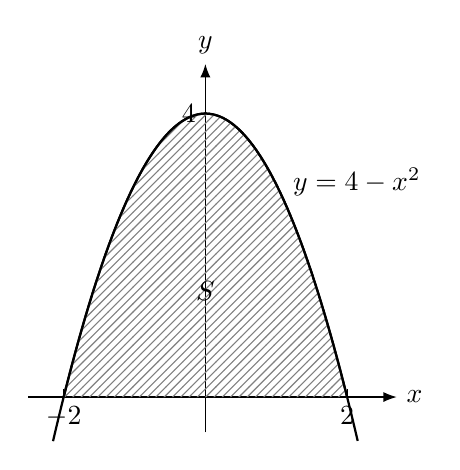
\begin{tikzpicture}[scale=0.9]
    % Axes
    \draw[-{Latex}] (-2.5,0) -- (2.7,0) node[right] {$x$};
    \draw[-{Latex}] (0,-0.5) -- (0,4.7) node[above] {$y$};
    % Parabola y=4-x^2
    \draw[thick,domain=-2.15:2.15,samples=100]
        plot (\x,{4-\x*\x});
    % Shaded area
    \path[pattern=north east lines,pattern color=gray]
        (-2,0) -- plot[domain=-2:2,samples=100] (\x,{4-\x*\x}) -- (2,0) -- cycle;
    % Re-draw boundary
    \draw[thick,domain=-2:2,samples=100]
        plot (\x,{4-\x*\x});
    \draw[dashed] (-2,0) -- (-2,0.15);
    \draw[dashed] (2,0) -- (2,0.15);
    \node[below] at (-2,0) {$-2$};
    \node[below] at (2,0) {$2$};
    \node[left] at (0,4) {$4$};
    \node at (0,1.5) {$S$};
    \node[above right] at (1.1,2.7) {$y=4-x^2$};
\end{tikzpicture}
\end{center}
Ta có $4-x^2=0$ khi $x=-2$ hoặc $x=2$. Vì $4-x^2\geq0$ trên $[-2,2]$:
\[
S=\int_{-2}^{2}(4-x^2)\,dx
=2\int_0^2(4-x^2)\,dx
=2\left(8-\frac{8}{3}\right)
=\frac{32}{3}.
\]

\subsubsection*{Ví dụ 2: Thể tích khối tròn xoay}
Cho miền giới hạn bởi $y=x$, trục $Ox$, $x=0$ và $x=2$. Khi quay miền này quanh $Ox$, ta được một khối tròn xoay có thể tích:

\begin{center}
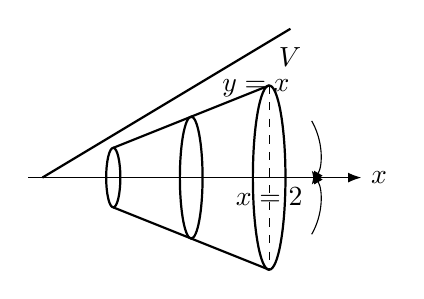
\begin{tikzpicture}[scale=0.9]
    % Axis
    \draw[-{Latex}] (-0.2,0) -- (4.5,0) node[right] {$x$};
    % Profile line y=x
    \draw[thick] (0,0) -- (3.5,2.1);
    % A few circular cross-sections
    \draw[thick] (1.0,0) ellipse (0.10 and 0.42);
    \draw[thick] (2.1,0) ellipse (0.16 and 0.86);
    \draw[thick] (3.2,0) ellipse (0.23 and 1.30);
    % Surface outline
    \draw[thick] (1.0,0.42) -- (2.1,0.86) -- (3.2,1.30);
    \draw[thick] (1.0,-0.42) -- (2.1,-0.86) -- (3.2,-1.30);
    \draw[dashed] (3.2,1.30) -- (3.2,-1.30);
    \node[below] at (3.2,0) {$x=2$};
    \node[above right] at (2.4,1.0) {$y=x$};
    \node[right] at (3.2,1.7) {$V$};
    \draw[-{Latex}] (3.8,0.8) arc (30:-30:0.9);
    \draw[-{Latex}] (3.8,-0.8) arc (-30:30:0.9);
\end{tikzpicture}
\end{center}
\[
V=\pi\int_0^2x^2\,dx
=\pi\left.\frac{x^3}{3}\right|_0^2
=\frac{8\pi}{3}.
\]

\subsection{2.2 Ứng dụng trong Vật lý và Cơ học}
\begin{itemize}
    \item \textbf{Tính quãng đường di chuyển:} Một vật chuyển động với vận tốc biến thiên theo thời gian $v(t)$ từ thời điểm $t_1$ đến $t_2$ sẽ đi được quãng đường $s$ là:
    \begin{equation}
    s = \int_{t_1}^{t_2} v(t) \, dt
    \end{equation}
    \item \textbf{Tính công của một lực:} Công $W$ sinh ra bởi một lực biến thiên $F(x)$ làm vật dịch chuyển từ $a$ đến $b$ dọc theo trục $Ox$ được tính bằng:
    \begin{equation}
    W = \int_{a}^{b} F(x) \, dx
    \end{equation}
\end{itemize}

\subsubsection*{Ví dụ 1: Tính quãng đường từ vận tốc}
Một ô tô chuyển động trên một đoạn đường với vận tốc
$v(t)=6t+2$ (m/s) trong khoảng thời gian từ $t=0$ đến $t=5$ s.

\begin{center}
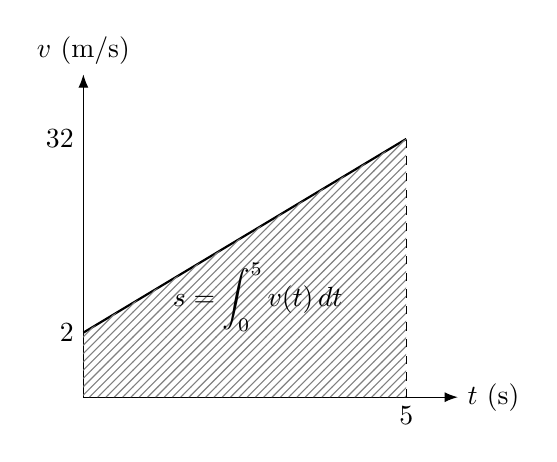
\begin{tikzpicture}[scale=0.82]
    \draw[-{Latex}] (0,0) -- (5.8,0) node[right] {$t$ (s)};
    \draw[-{Latex}] (0,0) -- (0,5.0) node[above] {$v$ (m/s)};
    \draw[thick] (0,1.0) -- (5,4.0);
    \path[pattern=north east lines,pattern color=gray]
        (0,0) -- (0,1.0) -- (5,4.0) -- (5,0) -- cycle;
    \draw[dashed] (5,0) -- (5,4.0);
    \node[below] at (5,0) {$5$};
    \node[left] at (0,1.0) {$2$};
    \node[left] at (0,4.0) {$32$};
    \node at (2.7,1.55) {$s=\displaystyle\int_0^5v(t)\,dt$};
\end{tikzpicture}
\end{center}
Quãng đường đi được là:
\[
s=\int_0^5(6t+2)\,dt
=\left.(3t^2+2t)\right|_0^5
=75+10=85\text{ m}.
\]

\subsubsection*{Ví dụ 2: Tính công của lực biến thiên}
Một lực tác dụng lên vật có dạng $F(x)=10+2x$ (N). Tính công khi vật di chuyển từ $x=0$ đến $x=5$ m:
\[
W=\int_0^5(10+2x)\,dx
=\left.(10x+x^2)\right|_0^5
=50+25=75\text{ J}.
\]

\subsection{2.3 Ứng dụng trong Kinh tế học}
Trong kinh tế học, tích phân được dùng để tính toán thặng dư của người tiêu dùng (Consumer Surplus - CS) và thặng dư của nhà sản xuất (Producer Surplus - PS) tại mức giá cân bằng thị trường $P_0$ và số lượng $Q_0$:
\begin{equation}
CS = \int_{0}^{Q_0} P_d(Q) \, dQ - P_0 Q_0
\end{equation}
\begin{equation}
PS = P_0 Q_0 - \int_{0}^{Q_0} P_s(Q) \, dQ
\end{equation}
Trong đó $P_d(Q)$ là hàm cầu và $P_s(Q)$ là hàm cung.

\begin{center}
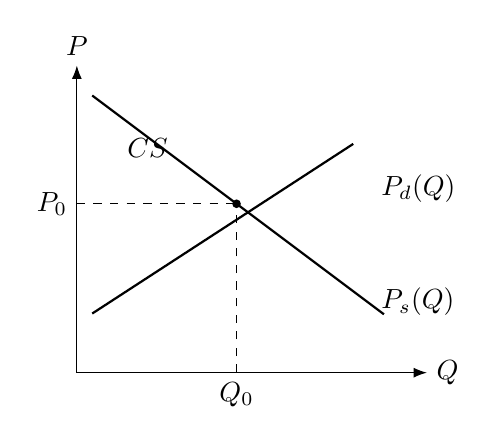
\begin{tikzpicture}[scale=0.78]
    \draw[-{Latex}] (0,0) -- (5.7,0) node[right] {$Q$};
    \draw[-{Latex}] (0,0) -- (0,5.0) node[above] {$P$};
    \draw[thick,domain=0.25:5.0] plot (\x,{4.7-0.75*\x});
    \draw[thick,domain=0.25:4.5] plot (\x,{0.8+0.65*\x});
    \draw[dashed] (2.6,0) -- (2.6,2.75);
    \draw[dashed] (0,2.75) -- (2.6,2.75);
    \fill (2.6,2.75) circle (2pt);
    \node[right] at (4.8,1.15) {$P_s(Q)$};
    \node[right] at (4.8,1.0+2.0) {$P_d(Q)$};
    \node[below] at (2.6,0) {$Q_0$};
    \node[left] at (0,2.75) {$P_0$};
    \node at (1.15,3.65) {$CS$};
\end{tikzpicture}
\end{center}

\subsubsection*{Ví dụ 1: Thặng dư của người tiêu dùng}
Giả sử hàm cầu của một sản phẩm là
\[
P_d(Q)=100-2Q
\]
và giá thị trường cân bằng là $P_0=60$, tương ứng với $Q_0=20$.
Khi đó:
\[
CS=\int_0^{20}(100-2Q)\,dQ-60\cdot20.
\]
Tính tích phân:
\[
CS=\left.(100Q-Q^2)\right|_0^{20}-1200
=1600-1200=400.
\]
Như vậy, thặng dư của người tiêu dùng là $400$ đơn vị tiền tệ.

\subsubsection*{Ví dụ 2: Thặng dư của nhà sản xuất}
Giả sử hàm cung là
\[
P_s(Q)=20+Q,
\]
với giá cân bằng $P_0=60$ và sản lượng $Q_0=40$.
Ta có:
\[
PS=60\cdot40-\int_0^{40}(20+Q)\,dQ.
\]
Suy ra:
\[
PS=2400-\left.(20Q+\frac{Q^2}{2})\right|_0^{40}
=2400-(800+800)=800.
\]
Vậy thặng dư của nhà sản xuất là $800$ đơn vị tiền tệ.

\section{Chương 3: Bài tập minh họa và Lời giải chi tiết}

\subsection{3.1 Bài toán tính diện tích hình phẳng}
\textbf{Đề bài:} Tính diện tích hình phẳng giới hạn bởi đường cong $y = x^2$ và đường thẳng $y = x + 2$. \\

\begin{center}
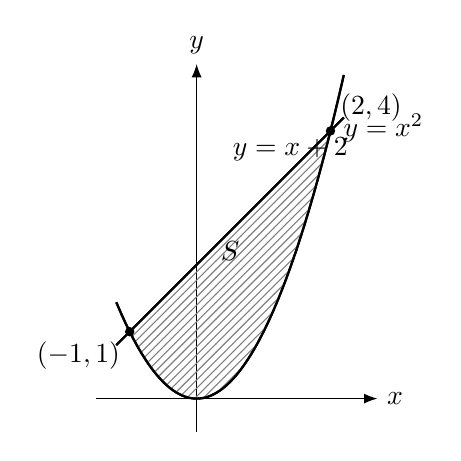
\begin{tikzpicture}[scale=0.85]
    \draw[-{Latex}] (-1.5,0) -- (2.7,0) node[right] {$x$};
    \draw[-{Latex}] (0,-0.5) -- (0,5.0) node[above] {$y$};
    \draw[thick,domain=-1.2:2.2,samples=100]
        plot (\x,{\x*\x});
    \draw[thick,domain=-1.2:2.2]
        plot (\x,{\x+2});
    \path[pattern=north east lines,pattern color=gray]
        (-1,1) -- plot[domain=-1:2,samples=100] (\x,{\x+2}) --
        (2,4) -- plot[domain=2:-1,samples=100] (\x,{\x*\x}) -- cycle;
    \draw[thick,domain=-1.2:2.2,samples=100]
        plot (\x,{\x*\x});
    \draw[thick,domain=-1.2:2.2]
        plot (\x,{\x+2});
    \fill (-1,1) circle (2pt);
    \fill (2,4) circle (2pt);
    \node[below left] at (-1,1) {$(-1,1)$};
    \node[above right] at (2,4) {$(2,4)$};
    \node[above] at (1.4,3.4) {$y=x+2$};
    \node[right] at (2.05,4.05) {$y=x^2$};
    \node at (0.5,2.2) {$S$};
\end{tikzpicture}
\end{center}
\textbf{Lời giải:}
Phương trình hoành độ giao điểm:
\[ x^2 = x + 2 \Leftrightarrow x^2 - x - 2 = 0 \Leftrightarrow x = -1 \text{ hoặc } x = 2 \]
Diện tích hình phẳng cần tìm là:
\[ S = \int_{-1}^{2} |x^2 - (x + 2)| \, dx = \int_{-1}^{2} (x + 2 - x^2) \, dx \]
\[ S = \left. \left( \frac{x^2}{2} + 2x - \frac{x^3}{3} \right) \right|_{-1}^{2} = \left( 2 + 4 - \frac{8}{3} \right) - \left( \frac{1}{2} - 2 + \frac{1}{3} \right) = \frac{9}{2} \]

\subsection{3.2 Bài toán tính công vật lý}
\textbf{Đề bài:} Một lò xo có độ cứng tự nhiên dài 10 cm. Lực cần thiết để kéo giãn nó thêm $x$ mét tuân theo định luật Hooke $F(x) = kx$. Biết rằng lực cần để giữ lò xo giãn ra thêm 2 cm là 40 N. Hãy tính công sinh ra khi kéo lò xo giãn từ 2 cm đến 6 cm. \\

\begin{center}
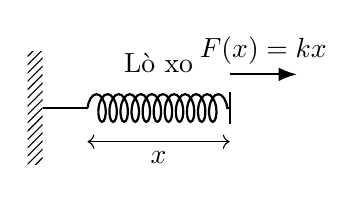
\begin{tikzpicture}[scale=0.95]
    % Wall and spring
    \fill[pattern=north east lines] (-0.15,-0.35) rectangle (0.05,1.15);
    \draw[thick] (0.05,0.4) -- (0.65,0.4);
    \draw[thick,decorate,decoration={coil,aspect=0.45,segment length=4pt,amplitude=5pt}]
        (0.65,0.4) -- (2.55,0.4);
    \draw[thick] (2.55,0.18) -- (2.55,0.62);
    \draw[-{Latex},thick] (2.55,0.85) -- (3.45,0.85);
    \node[above] at (3.0,0.85) {$F(x)=kx$};
    \draw[<->] (0.65,-0.05) -- (2.55,-0.05);
    \node[below] at (1.6,-0.05) {$x$};
    \node at (1.6,1.0) {Lò xo};
\end{tikzpicture}
\end{center}
\textbf{Lời giải:}
Đổi đơn vị: $2 \text{ cm} = 0.02 \text{ m}$. Ta có $F(0.02) = k \cdot 0.02 = 40 \Rightarrow k = 2000 \text{ N/m}$. \\
Hàm lực là $F(x) = 2000x$. \\
Công cần thiết để kéo giãn lò xo từ $2 \text{ cm} = 0.02 \text{ m}$ đến $6 \text{ cm} = 0.06 \text{ m}$ là:
\begin{align*}
W&=\int_{0.02}^{0.06}2000x\,dx\\
 &=\left.1000x^2\right|_{0.02}^{0.06}\\
 &=1000(0.06^2-0.02^2)\\
 &=1000(0.0036-0.0004)=3.2\text{ J}.
\end{align*}


\subsection{3.3 Bài toán tính thể tích khối tròn xoay}
\textbf{Đề bài:} Tính thể tích khối tạo thành khi quay miền giới hạn bởi
$y=x^2$, trục $Ox$, $x=0$ và $x=1$ quanh trục $Ox$.\\
\textbf{Lời giải:}
Theo công thức thể tích vật thể tròn xoay:
\[
V=\pi\int_0^1(x^2)^2\,dx
=\pi\int_0^1x^4\,dx
=\pi\left.\frac{x^5}{5}\right|_0^1
=\frac{\pi}{5}.
\]

\subsection{3.4 Bài toán tính quãng đường chuyển động}
\textbf{Đề bài:} Một vật chuyển động với vận tốc
$v(t)=4t^2+2$ (m/s). Tính quãng đường vật đi được trong $3$ giây đầu.\\
\textbf{Lời giải:}
\[
s=\int_0^3(4t^2+2)\,dt
=\left.\left(\frac{4}{3}t^3+2t\right)\right|_0^3
=36+6=42\text{ m}.
\]

\subsection{3.5 Bài toán tích phân từng phần}
\textbf{Đề bài:} Tính tích phân
\[
I=\int_1^e\ln x\,dx.
\]
\textbf{Lời giải:}
Chọn $u=\ln x$, $dv=dx$, suy ra $du=\frac{1}{x}dx$ và $v=x$.
Do đó:
\[
I=\left.x\ln x\right|_1^e-\int_1^e1\,dx
=e-(e-1)=1.
\]

\section*{Kết luận}
\addcontentsline{toc}{section}{Kết luận}
Qua tiểu luận này, chúng ta thấy rõ tích phân không đơn thuần là các phép tính toán lý thuyết khan hiếm trên giảng đường, mà là một chiếc chìa khóa vạn năng giúp giải quyết những bài toán phức tạp trong thực tế đời sống. Việc nắm vững cả lý thuyết cốt lõi lẫn phương pháp ứng dụng thực tiễn sẽ tạo nền tảng vững chắc cho sinh viên trong các môn học chuyên ngành tiếp theo.

\section*{Tài liệu tham khảo}
\addcontentsline{toc}{section}{Tài liệu tham khảo}
\begin{enumerate}
    \item Nguyễn Đình Trí (Chủ biên), \textit{Toán học cao cấp - Tập 2: Giải tích}, NXB Giáo dục Việt Nam.
    \item James Stewart, \textit{Calculus: Early Transcendentals}, Cengage Learning.
    \item Các bài giảng giải tích trực tuyến và tài liệu tham khảo nội bộ.
\end{enumerate}

\end{document}
